% Created 2022-04-08 Fri 12:12
% Intended LaTeX compiler: pdflatex
\documentclass[presentation]{beamer}
\usepackage[utf8]{inputenc}
\usepackage[T1]{fontenc}
\usepackage{graphicx}
\usepackage{grffile}
\usepackage{longtable}
\usepackage{wrapfig}
\usepackage{rotating}
\usepackage[normalem]{ulem}
\usepackage{amsmath}
\usepackage{textcomp}
\usepackage{amssymb}
\usepackage{capt-of}
\usepackage{hyperref}
\usetheme[progressbar=foot]{metropolis}
\author{Edmund Miller}
\date{\today}
\title{Current Research}
\hypersetup{
 pdfauthor={Edmund Miller},
 pdftitle={Current Research},
 pdfkeywords={},
 pdfsubject={},
 pdfcreator={Emacs 29.0.50 (Org mode 9.6)}, 
 pdflang={English}}
\makeatletter
\newcommand{\citeprocitem}[2]{\hyper@linkstart{cite}{citeproc_bib_item_#1}#2\hyper@linkend}
\makeatother

\usepackage[notquote]{hanging}
\begin{document}

\maketitle

\section*{Background}
\label{sec:org02c0ebf}
\section*{Enhancer intro}
\label{sec:orga79c09e}
\begin{frame}[label={sec:org8013042}]{Central Dogma of Biology}
\begin{center}
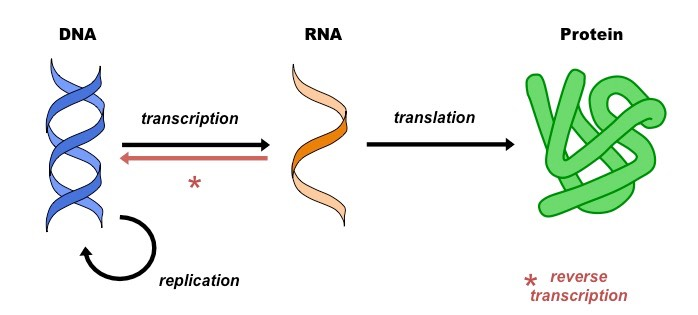
\includegraphics[width=.9\linewidth]{/home/emiller/src/personal/edmundmiller-dev/static/org-attach/b8/ce871b-5b7f-4cef-b389-7b27459818b3/_20220407_195627screenshot.png}
\end{center}
\end{frame}

\begin{frame}[label={sec:orgf168fd4}]{A Simple View of Gene Expression}
\begin{columns}
\begin{column}{0.45\columnwidth}
\begin{block}{Gene Expression}
\begin{center}
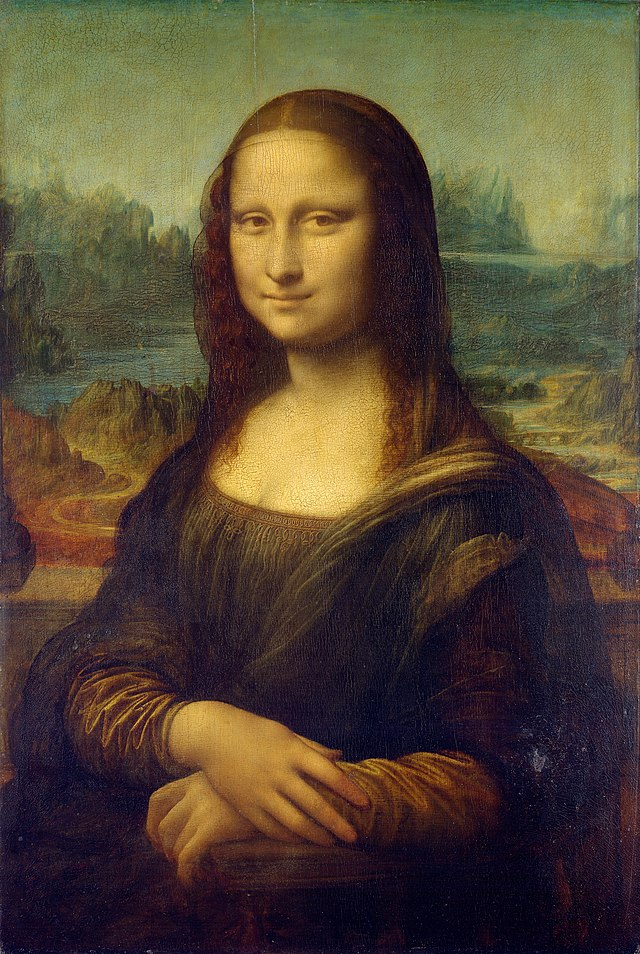
\includegraphics[width=.9\linewidth]{/home/emiller/src/personal/edmundmiller-dev/static/org-attach/a9/ae81d7-3773-4daa-baf6-bec17b6bb120/_20220407_195540screenshot.png}
\end{center}
\end{block}
\end{column}


\begin{column}{0.45\columnwidth}
\begin{block}{Central Dogma}
\begin{center}
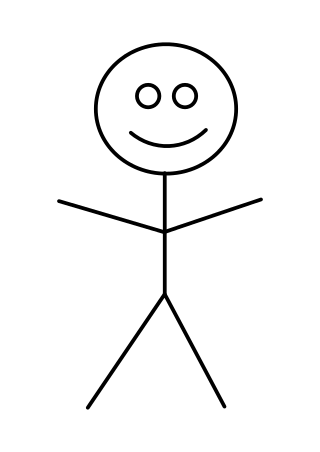
\includegraphics[width=.9\linewidth]{/home/emiller/src/personal/edmundmiller-dev/static/org-attach/a9/ae81d7-3773-4daa-baf6-bec17b6bb120/_20220407_195803screenshot.png}
\end{center}
\end{block}
\end{column}
\end{columns}
\end{frame}


\begin{frame}[label={sec:orgefc5d0a}]{Enhancers Image}
\end{frame}

\begin{frame}[label={sec:orgd4d70ba}]{Enhancers Fun facts}
\begin{itemize}
\item Cis-acting DNA sequences that can increase the transcription of genes \footnote{(Pennacchio et al. 2013)\label{org986cd75}}
\end{itemize}
\end{frame}

\begin{frame}[label={sec:org268bda8}]{Multiple Enhancers can regulate one gene}
\begin{figure}[htbp]
\centering
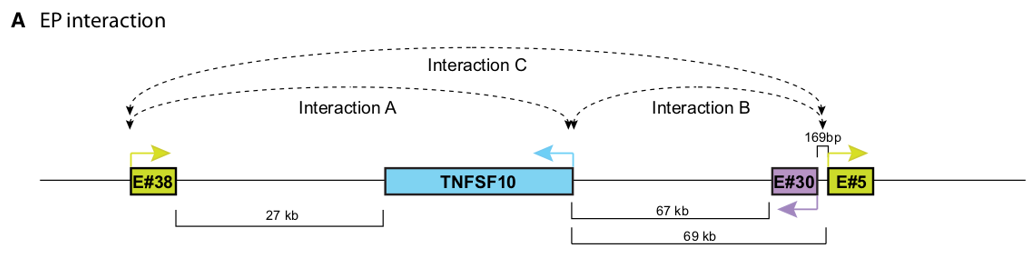
\includegraphics[width=.9\linewidth]{/home/emiller/src/personal/edmundmiller-dev/static/org-attach/41/914259-ccb3-42b6-a38e-7e284c0bdded/_20220408_094258screenshot.png}
\caption[Short caption]{[fn:1: (Kim et al. 2018)]}
\end{figure}
\end{frame}


\begin{frame}[label={sec:org60c8203}]{Enhancers can regulate multiple genes}
\end{frame}
\begin{frame}[label={sec:org22c6014}]{Topologically Associating Domain (TAD)}
\end{frame}
\begin{frame}[label={sec:orgb6d85ad}]{Why are Enhancers difficult to identify?}
\begin{itemize}
\item Scattered across the 98\% of the human genome that does not encode proteins \textsuperscript{\ref{org986cd75}}
\item Enhancers location relative to their target gene (or genes) is highly
variable. They can be upstream, downstream, or within introns. \textsuperscript{\ref{org986cd75}}
\item Enhancers do not necessarily act on the respective closest promoter but can
bypass neighbouring genes to regulate genes located more distantly along a
chromosome\textsuperscript{\ref{org986cd75}}
\end{itemize}
\end{frame}

\begin{frame}[label={sec:orge2681cf}]{eRNAs Introduction}
\end{frame}

\begin{frame}[label={sec:org8a56f61}]{Global Transcriptional Activity dynamics reveal functional enhancer rnas}
\begin{block}{GRO-seq Overview}
\begin{figure}[htbp]
\centering
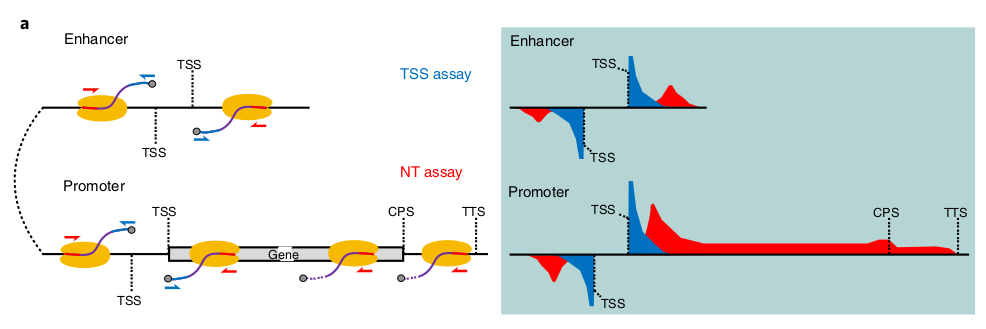
\includegraphics[width=.9\linewidth]{/home/emiller/src/personal/edmundmiller-dev/static/org-attach/08/136bc2-5fce-4dbb-bdb3-14793c5261d3/_20220408_111821screenshot.png}
\caption{(Yao et al. 2022)}
\end{figure}
\end{block}


\begin{block}{Reproduction with IMR}
\end{block}
\end{frame}
\section*{Hypothesis}
\label{sec:org9f34125}
\section*{Aims}
\label{sec:org5bba25c}
\begin{frame}[label={sec:org1c1b472}]{Aim 1 Create a best practice secondary analysis pipeline for nascent transcripts}
\end{frame}
\begin{frame}[label={sec:org36a2a0a}]{Aim 2 Take advantage of New Developments to improve eRNA annotation}
\begin{block}{New developments}
\end{block}
\begin{block}{CHM13}
\begin{block}{\href{https://pubmed.ncbi.nlm.nih.gov/35357915/}{Epigenetic patterns in a complete human genome - PubMed}}
\end{block}
\end{block}
\begin{block}{PINTS}
\begin{block}{NT vs TSS}
\begin{figure}[htbp]
\centering
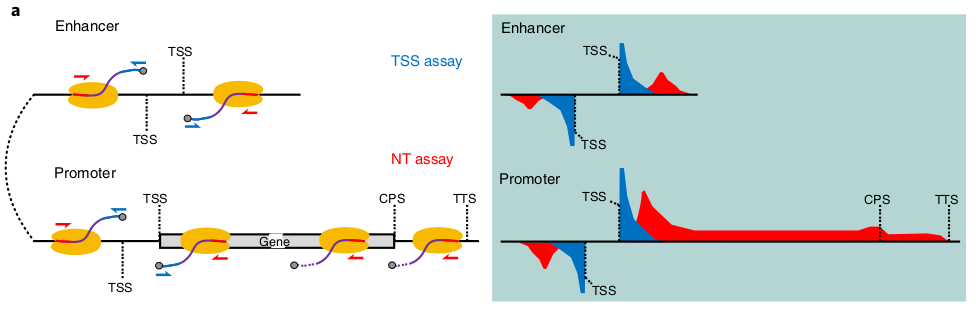
\includegraphics[width=.9\linewidth]{/home/emiller/src/personal/edmundmiller-dev/static/org-attach/cb/525ffe-5925-48af-a434-cff675b835be/_20220408_112049screenshot.png}
\caption{(Yao et al. 2022)}
\end{figure}
\end{block}


\begin{block}{Can we use this for NT assays?}
\end{block}
\end{block}
\end{frame}
\begin{frame}[label={sec:org54035df}]{Aim 3 Compare eRNA dynamics between cell lines}
\end{frame}
\end{document}
